\clearpage

\begin{appendices}

\section{Templates}
\subsection{Figures}
\begin{figure}[h!]
\centering
  \minipage{0.3\textwidth}
    \fbox{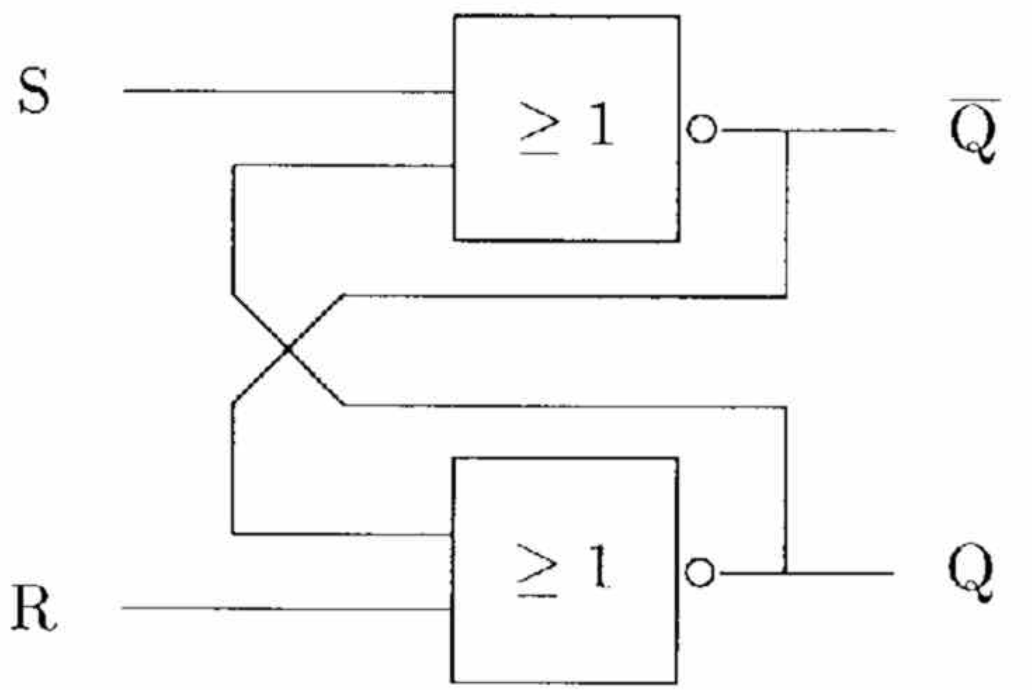
\includegraphics[height=2.5cm, keepaspectratio]{images/rsflipflop.png}}%
    \caption{RS-Flipflop}%
    \label{fig:rsflipflop}
  \endminipage\hspace{1cm}   
%
  \minipage{0.4\textwidth}
    \fbox{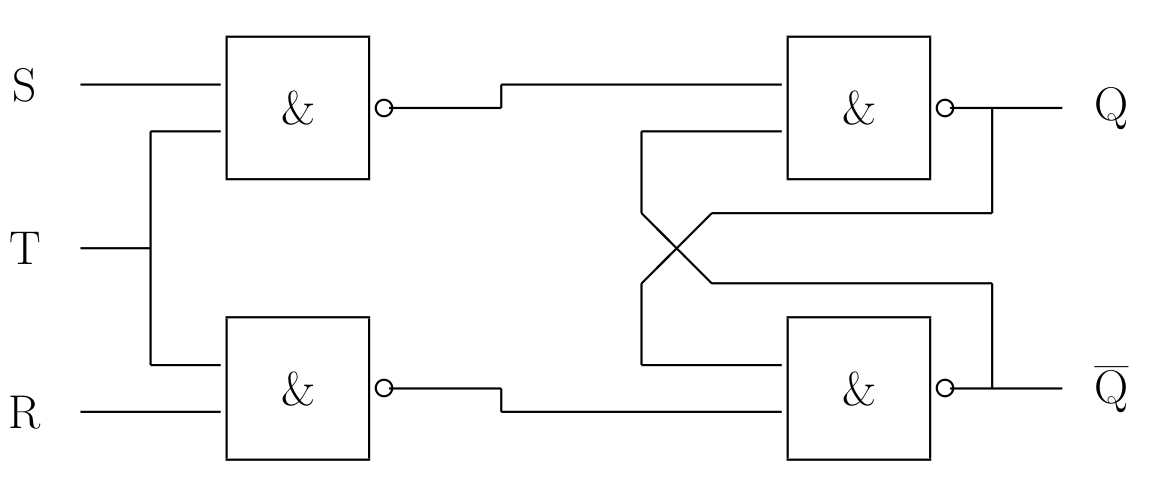
\includegraphics[height=2.5cm, keepaspectratio]{images/rsflipfloptakt.png}}%
    \caption{getaktetes RS-Flipflop}%
    \label{fig:rsflipfloptakt}
  \endminipage
\end{figure}

Referencing: Figure \ref{fig:rsflipflop}, Figure \ref{fig:rsflipfloptakt}).



Fusce suscipit mauris a justo dignissim, sit amet cursus lacus blandit. Aenean quis interdum ipsum. Integer scelerisque lacus eu lacinia vulputate. Nunc vitae pulvinar nisi. In eget pulvinar ante. Donec ultrices nec erat non porta. Ut feugiat ligula et finibus rutrum. Cras varius congue sapien, id pulvinar mi fringilla et.
%
\piccaption{Darstellung des Zahlenbereichs des Zweierkomplements mit acht Stellen\label{fig:tabelle_zweierkomplement}}
\parpic[r]{%
	\fbox{
		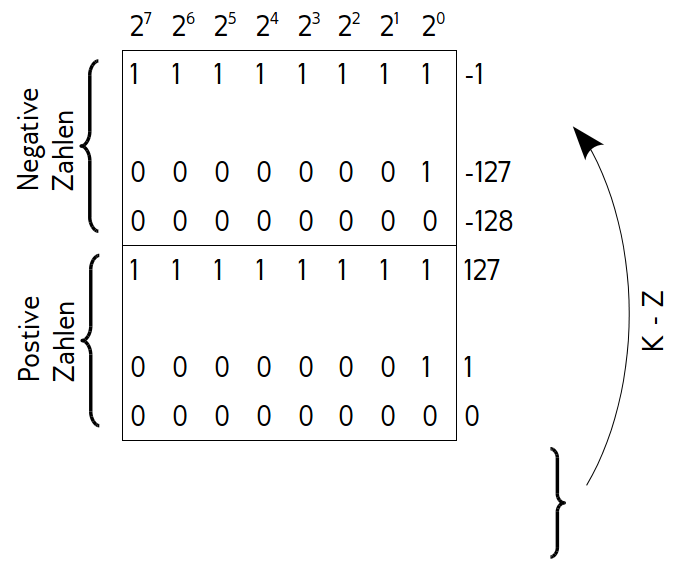
\includegraphics[width = 5.5cm, keepaspectratio]{images/tabelle_zweierkomplement.png}
	}
}
%
Lorem ipsum dolor sit amet, consectetur adipiscing elit. Vivamus sodales cursus finibus. Vestibulum ante ipsum primis in faucibus orci luctus et ultrices posuere cubilia Curae; Vestibulum sagittis faucibus felis ut efficitur. Donec vel pretium enim. Nulla ut urna facilisis, fringilla mauris id, aliquam arcu. Pellentesque tincidunt dapibus aliquet. Aliquam iaculis, risus molestie efficitur ultrices, nibh sapien mattis urna, non iaculis dolor mauris a nisl. Nam imperdiet, dui sit amet vestibulum rutrum, justo massa luctus magna, a aliquet risus ligula ultricies erat. Ut fermentum volutpat arcu ac auctor. In condimentum vehicula placerat. Nunc placerat eros id eros sagittis, et auctor lacus blandit. Donec blandit est nec sapien faucibus dapibus.

\subsection{Tables}
\begin{center}
	\begin{tabular}[c]{c | c | c || c| c | c || c | c || c | c | c || c| c| c}
		\multicolumn{3}{c||}{Konjunktion}	&	\multicolumn{3}{c||}{Disjunktion} & \multicolumn{2}{c||}{Negation} & \multicolumn{3}{c||}{NAND} & \multicolumn{3}{c}{NOR}\\
		\multicolumn{3}{c||}{UND}	&	\multicolumn{3}{c||}{ODER} & \multicolumn{2}{c||}{} & \multicolumn{3}{c||}{} & \multicolumn{3}{c}{}\\
		\hline
		$a$ & $b$ & $a$ $\wedge$ $b$ & $a$ & $b$ & $a$ $\vee$ $b$ & $a$ & $\bar{a}$ & $a$ & $b$ & $\overline{a \wedge b}$ & $a$ & $b$ & $\overline{a \vee b}$\\
		\hline
		0 & 0 & 0 & 0 & 0 & 0 & 0 & 1 & 0 & 0 & 1 & 0 & 0 & 1\\
		0 & 1 & 0 & 0 & 1 & 1 & 1 & 0 & 0 & 1 & 1 & 0 & 1 & 0\\
		1 & 0 & 0 & 1 & 0 & 1 & & & 1 & 0 & 1 & 1 & 0 & 0\\
		1 & 1 & 1 & 1 & 1 & 1 & & & 1 & 1 & 0 & 1 & 1 & 0\\
		\hline
	\end{tabular}
\end{center}

\end{appendices}